\chapter{Results}\label{ch:results}

Results text here.

\section{Hückel Approximation}\label{sec:huckelmethodresults}

\begin{figure}[h!]
\begin{center}
\hspace*{-2.7cm}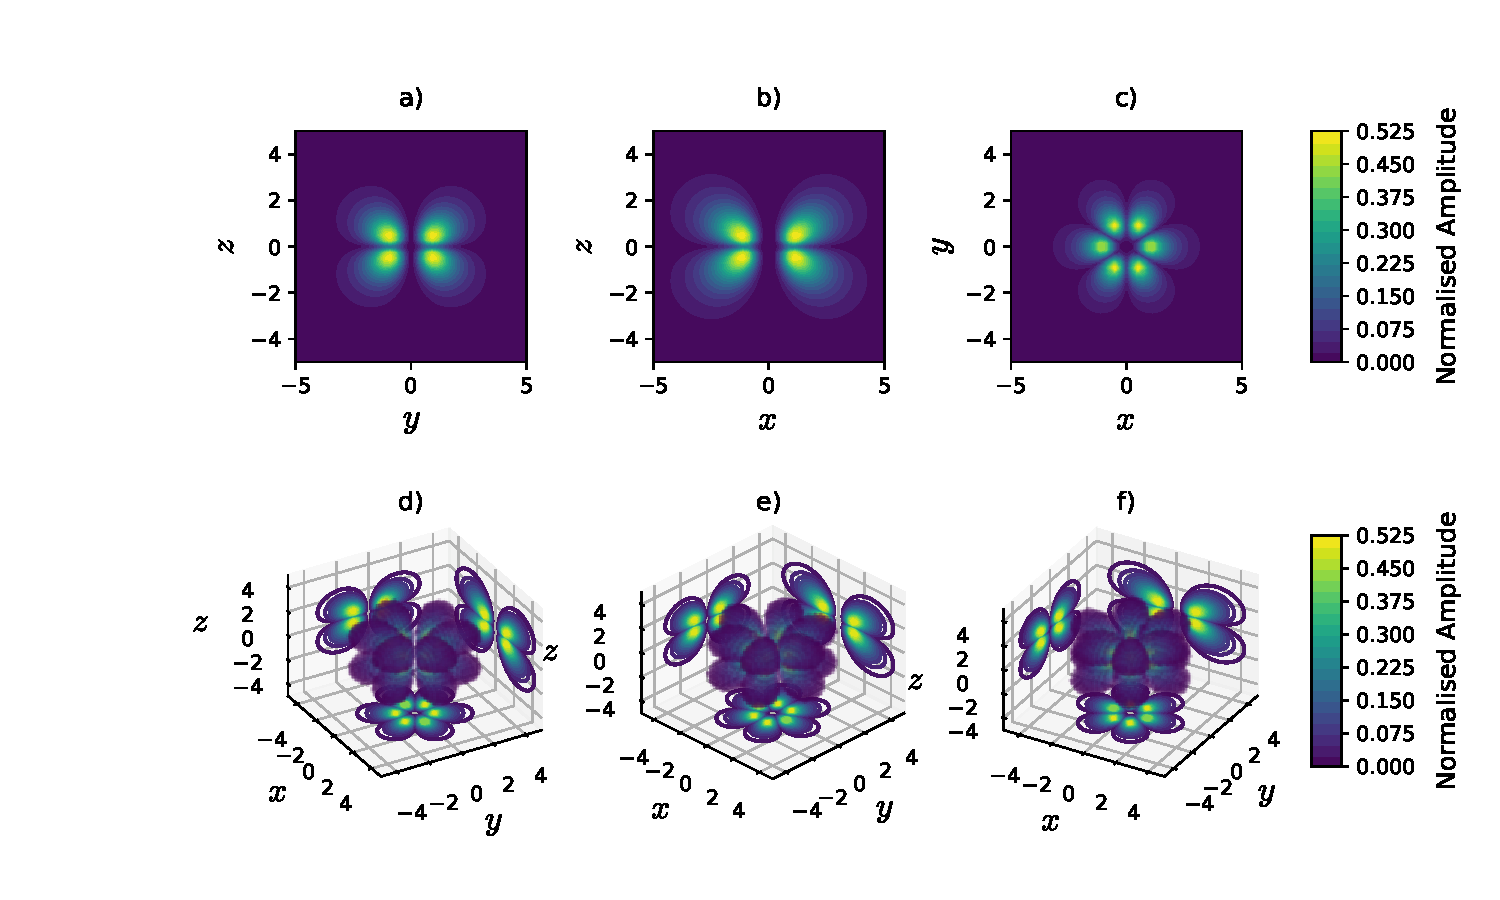
\includegraphics[width=1.2\linewidth]{figures/Figure1.pdf}
\end{center}
\caption{Orbital electron wavefunction of Benzene, using the Hückel approximation with orbital angular momentum quantum numbers l=1 and m=0.}
\label{fig:random_matrix}
\end{figure} 


\section{Hartree-Fock Analytical Approximation}\label{sec:hartreeanalyticresults}
\section{Hartree-Fock Numerical Approximation}\label{sec:hartreenumericalresults}
\section{Many-Body Electron Perturbations}\label{sec:electronperturbationresults}
\section{GLSL High-Order Perturbations}\label{sec:GLSLhighorderresults}